\documentclass[11pt]{amsart}
\usepackage[margin=1.15in]{geometry}
\usepackage{amssymb,amsmath,mathtools}
\usepackage{graphicx}
\usepackage[hidelinks]{hyperref}
\usepackage[expansion=false]{microtype}

\newtheorem{theorem}{Theorem}[section]
\newtheorem{proposition}[theorem]{Proposition}
\newtheorem{lemma}[theorem]{Lemma}
\newtheorem{corollary}[theorem]{Corollary}
\newtheorem{mainthm}{Theorem}
\renewcommand{\themainthm}{\Alph{mainthm}}
\theoremstyle{definition}
\newtheorem{definition}[theorem]{Definition}
\newtheorem{remark}[theorem]{Remark}
\newtheorem{question}[theorem]{Question}

\newcommand{\ZZ}{\mathbb{Z}}
\newcommand{\one}{\mathbf 1}
\newcommand{\Nmin}{N_{\min}}
\newcommand{\B}{\mathsf B}
\newcommand{\zenodoCodeDOI}{10.5281/zenodo.XXXXXXX}

\setlength{\emergencystretch}{2.5em}
\hbadness=2000
\raggedbottom
\begin{document}

\title[Dhar's minimal sand conjecture]{Proof of Dhar's Minimal Sand Conjecture\\ for the Manna Sandpile}

\author{Deep Bhattacharjee}
\address{Formerly, Electro-Gravitational Space Propulsion Laboratory (EGSPL), Bhubaneswar, Odisha 751030, India}
\address{Formerly, University of Calcutta (Heramba Chandra College), 23/49 Gariahat Road, Golpark, Kolkata 700029, West Bengal, India}
\email{d.bhattacharjee@erl-forschung.de}
\email{itsdeep@live.com}
\email{egspl@proton.me (GitHub-related contact; GitHub account creelie)}
\urladdr{https://orcid.org/0000-0003-0466-750X}

\begin{abstract}
In 1999 Dhar conjectured that every recurrent configuration of Manna's stochastic sandpile on an $\ell\times m$ rectangle carries at least $\lceil(\ell-1)(m-1)/2\rceil$ grains, and showed that this number is attained. We prove the conjecture. In $d$ dimensions the same argument gives the exact minimum whenever at least $d-1$ side lengths of the box are odd.

\medskip\noindent\textbf{Keywords:} Manna sandpile; recurrent configurations; self-organized criticality.

\smallskip\noindent\textbf{MSC 2020:} 82C20 (primary); 05C57, 60J10.
\end{abstract}

\maketitle

\section{Introduction}\label{sec:intro}

Manna's sandpile \cite{Man91} is the simplest sandpile in which the toppling rule is random. Grains are dropped one at a time on the sites of a rectangle. A site holding two or more grains topples: it gives away two grains, either one to each of its horizontal neighbours or one to each of its vertical neighbours, the direction being chosen by a fair coin. Grains pushed across the boundary are lost. Like the deterministic sandpile of Bak, Tang and Wiesenfeld \cite{BTW87,BTW88} and its abelian form \cite{Dha90}, the model settles into a stationary state, and the configurations that occur in it with positive probability are called recurrent. Dhar showed that the particle addition operators of the Manna model commute \cite{Dha99a,Dha99b}, which places the model among the abelian networks studied later in a general setting \cite{BL16}, and he found that the recurrent configurations obey local constraints: two by two blocks of empty sites, and many larger patterns, never occur \cite{Dha99b}.\footnote{Dhar called such patterns forbidden subconfigurations. For the deterministic sandpile they are exactly the patterns detected by the burning algorithm \cite{MD92,Dha90}; for the Manna model no comparable test is known \cite[\S5]{Dha99b}.}

Let $\Nmin(\ell,m)$ be the least number of grains in a recurrent configuration of the Manna model on the $\ell\times m$ rectangle. Dhar proved that $\Nmin(\ell,m)\le f(\ell,m)$, where
\begin{equation}\label{eq:f}
f(\ell,m)=\begin{cases}\tfrac12(\ell-1)(m-1), & \ell\text{ or }m\text{ odd},\\[2pt] \tfrac12(\ell m-\ell-m+2), & \ell\text{ and }m\text{ even},\end{cases}
\end{equation}
checked equality for $\ell,m\le4$ and for $\ell\le 2$, and conjectured that $\Nmin=f$ for all rectangles; a proof, he wrote, ``remains an open problem'' \cite[\S6]{Dha99b}. For the limiting density $\rho_{\min}=\lim\Nmin(\ell,m)/\ell m$ he proved $\rho_{\min}\ge\tfrac14$, $\tfrac27$ and $\tfrac13$, by tiling the plane with $2\times2$ squares and with tiles of $7$ and $12$ sites inside which every configuration with too few grains contains a forbidden pattern; the conjecture gives $\rho_{\min}=\tfrac12$. The two cases of \eqref{eq:f} are one formula: $(\ell-1)(m-1)$ is even unless $\ell$ and $m$ are both even, and in that case $\tfrac12(\ell m-\ell-m+2)=\tfrac12\bigl((\ell-1)(m-1)+1\bigr)$. Thus
\begin{equation}\label{eq:fceil}
f(\ell,m)=\Bigl\lceil \tfrac12(\ell-1)(m-1)\Bigr\rceil,
\end{equation}
which is half the number of unit squares of the rectangle, rounded up.

\begin{mainthm}\label{thm:A}
For all $\ell,m\ge1$, every recurrent configuration of the Manna model on the $\ell\times m$ rectangle has at least $\lceil(\ell-1)(m-1)/2\rceil$ grains, and this bound is attained. That is, $\Nmin(\ell,m)=f(\ell,m)$.
\end{mainthm}

The model has a natural version on the box $[\ell_1]\times\dots\times[\ell_d]$ of $\ZZ^d$, where $[n]=\{1,\dots,n\}$: an unstable site chooses one of the $d$ axes uniformly at random and sends one grain to each of its two neighbours along that axis. Write $\Nmin(\ell_1,\dots,\ell_d)$ for the least number of grains in a recurrent configuration.

\begin{mainthm}\label{thm:B}
Every recurrent configuration of the $d$-dimensional Manna model on $[\ell_1]\times\dots\times[\ell_d]$ has at least
\[
\Bigl\lceil 2^{1-d}\prod_{i=1}^d(\ell_i-1)\Bigr\rceil
\]
grains. If at least $d-1$ of the numbers $\ell_1,\dots,\ell_d$ are odd, the bound is attained, and $\Nmin(\ell_1,\dots,\ell_d)=2^{1-d}\prod_i(\ell_i-1)$.
\end{mainthm}

For $d=2$ the lower bound is the bound of Theorem~\ref{thm:A}, and the second statement covers the rectangles with an odd side. The lower bound is not attained on every box. When a side has length two, an edge lies in fewer cells than the count assumes, and the same argument gives more; on the $4\times2\times2$ box the minimum is $2$, while the bound of Theorem~\ref{thm:B} is $1$. Theorem~\ref{thm:two} in Section~\ref{sec:remarks} gives the sharper bound and its exact value on a family of such boxes. The minimal density of grains in recurrent configurations is therefore $2^{1-d}$ in dimension $d$, and $\tfrac12$ in the plane, as Dhar predicted \cite[(24)]{Dha99b}.

\subsection*{The idea}
The lower bound comes from one observation about the order in which sites topple for the last time. Run the sandpile from the full configuration to a recurrent configuration $z$, and look at a unit square of the rectangle. Among its four corners, take the one, $w$, whose last toppling happened latest. At that toppling $w$ sent a grain to one of its two neighbours inside the square, say $u$, and $u$ had already toppled for the last time. That grain is still at $u$ at the end. So every unit square has a grain sitting on one of its corners, delivered along one of its edges, and an edge borders only two squares. Counting gives half the number of squares (Figure~\ref{fig:square}). The argument never needs to know which configurations are recurrent; it uses only that a recurrent configuration is the end point of some legal history. The upper bound is Dhar's construction \cite[\S6]{Dha99b}, which adds two columns at a time. We write it out in full, check that the histories it uses can be realized by the Markov chain, and carry it to $d$ dimensions, where a $(d-1)$-dimensional layer plays the part of the column.

\begin{figure}[t]
\centering
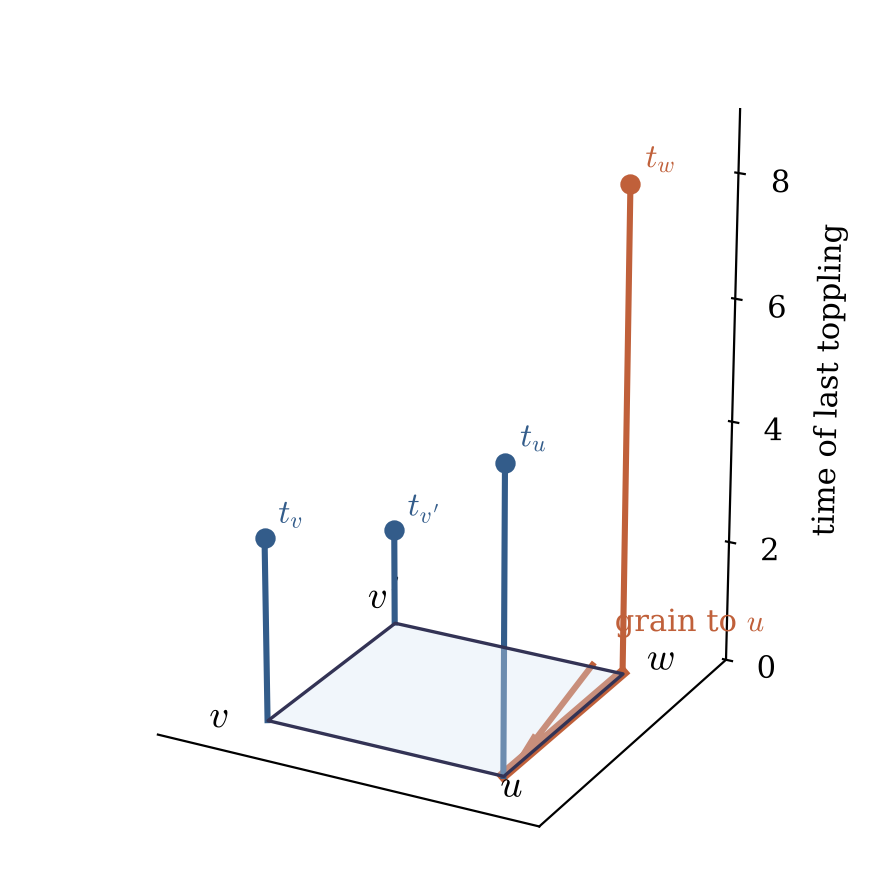
\includegraphics[width=0.62\textwidth]{fig_square.png}
\caption{The key step. The four corners of a unit square carry the times of their last topplings. The corner $w$ with the latest one sends, at that moment, a grain along an edge of the square to a corner $u$ that will never topple again, so the grain stays at $u$.}\label{fig:square}
\end{figure}

\subsection*{Plan}
Section~\ref{sec:model} defines the model and proves three facts used throughout: stabilization terminates, recurrence means reachability from the full configuration, and any legal history between stable configurations can be realized by the chain. Section~\ref{sec:last} records what a history implies about last topplings. Section~\ref{sec:lower} proves the lower bounds, including a local form valid in every sub-box. Section~\ref{sec:upper} gives the constructions and completes the proofs of Theorems~\ref{thm:A} and~\ref{thm:B}. Section~\ref{sec:remarks} treats boxes with a side equal to $3$ or $2$, the minimal density in general boxes, cylinders and the remaining open cases, and comments on Dhar's paper. Appendix~\ref{app:check} describes an independent exhaustive check on small rectangles.

\section{The model}\label{sec:model}

Fix $d\ge1$ and a box $\B=[\ell_1]\times\dots\times[\ell_d]\subset\ZZ^d$. Let $e_1,\dots,e_d$ be the unit vectors. Two sites $s,t\in\B$ are neighbours along axis $i$ if $t=s\pm e_i$; the edge $\{s,t\}$ then has axis $i$. A configuration is a map $z\colon\B\to\ZZ_{\ge0}$; $z(s)$ is the number of grains at $s$. It is stable if $z(s)\le1$ for every $s$. The full configuration is $\one$, with $z\equiv1$.

Two operations change a configuration. An \emph{addition} at $s$ increases $z(s)$ by one. A \emph{toppling} of $s$ along axis $i$ decreases $z(s)$ by two and increases $z(s-e_i)$ and $z(s+e_i)$ by one each, for those of the two sites that lie in $\B$; a grain sent to a point outside $\B$ is lost. A toppling of $s$ is \emph{legal} if $z(s)\ge2$ just before it. A \emph{legal history} from $z$ to $z'$ is a finite sequence of additions and legal topplings that transforms $z$ into $z'$. Intermediate configurations may be unstable, and additions may be made while some sites are unstable.

\begin{lemma}\label{lem:finite}
Let $A$ be a nonempty set of axes. Starting from any configuration, every sequence of legal topplings, all along axes in $A$ and with no additions, is finite.
\end{lemma}

\begin{proof}
Topplings do not increase the total number of grains $G$, so no height ever exceeds $G$. Suppose an infinite sequence of legal topplings exists. Some site $s_0$ topples infinitely often, and along some axis $i_0\in A$ infinitely often. Each such toppling sends a grain to $s_0-e_{i_0}$. If $s_0-e_{i_0}\in\B$, that site receives infinitely many grains; since its height stays at most $G$, it topples infinitely often, and we call it $s_1$ and choose an axis $i_1\in A$ along which it topples infinitely often. Continuing, we obtain sites $s_0,s_1,\dots$ whose coordinate sums strictly decrease, so the process stops at some $s_k$ with $s_k-e_{i_k}\notin\B$. Then each of the infinitely many topplings of $s_k$ along $i_k$ sends a grain out of $\B$, and $G$ decreases infinitely often, which is impossible because $G$ is a nonnegative integer that never increases.
\end{proof}

\subsection{The Markov chain}
Fix a total order on $\B$ and numbers $p_s>0$ with $\sum_sp_s=1$. From a stable configuration, one step of the chain adds a grain at a site chosen with probability $p_s$ and then, as long as some site is unstable, topples the smallest unstable site along an axis chosen uniformly at random, independently of everything else. By Lemma~\ref{lem:finite} with $A=\{1,\dots,d\}$ this ends in a stable configuration, so the chain lives on the finite set of stable configurations. For $d=2$ this is Dhar's formulation of Manna's model \cite[\S2]{Dha99b}.\footnote{Dhar lets each site draw its directions from its own sequence of random numbers, which makes the order of topplings irrelevant. The order fixed here does not affect any statement below: the stationary support is characterized in Lemma~\ref{lem:recurrent} without reference to it, and Lemma~\ref{lem:realize} holds for any order.} A stable configuration is \emph{recurrent} if it has positive probability in a stationary distribution, and $\Nmin(\ell_1,\dots,\ell_d)$ is the least number of grains of a recurrent configuration.

\begin{lemma}\label{lem:recurrent}
The chain has a unique stationary distribution. A stable configuration is recurrent if and only if the chain reaches it from $\one$ with positive probability.
\end{lemma}

\begin{proof}
From any stable configuration the chain reaches $\one$ with positive probability: it suffices to add grains, one at a time, at the empty sites, which causes no toppling. Let $R$ be the set of stable configurations reachable from $\one$. Every element of $R$ leads back to $\one$, so $R$ is a communicating class, and it is closed, since anything reachable from an element of $R$ is reachable from $\one$. Restricted to $R$ the chain is irreducible, so it has exactly one stationary distribution supported in $R$, and this distribution is positive at every element of $R$ \cite[\S1.7]{Nor97}. It remains to see that every stationary distribution $\pi$ vanishes outside $R$. From each stable configuration the chain enters $R$ within $K=|\B|$ steps with probability at least some $\varepsilon>0$, by the additions just described, and once in $R$ it stays there. Hence the probability of remaining outside $R$ for $nK$ steps is at most $(1-\varepsilon)^n$ from any starting point, and stationarity gives $\pi(\mathcal S\setminus R)\le(1-\varepsilon)^n$ for every $n$, where $\mathcal S$ is the set of stable configurations. So $\pi(\mathcal S\setminus R)=0$, and $\pi$ is the stationary distribution of the chain on $R$.
\end{proof}

The chain makes additions only at stable configurations and topples in a prescribed order. The constructions of Section~\ref{sec:upper} are more convenient as legal histories, and the next lemma shows that nothing is lost. It is the least action principle for abelian networks \cite{FLP10,BL16}; we give the short proof for the model at hand.

\begin{lemma}\label{lem:realize}
Let $z,z'$ be stable configurations. If there is a legal history from $z$ to $z'$, the chain started at $z$ reaches $z'$ with positive probability.
\end{lemma}

\begin{proof}
Let $\mathcal H$ be a legal history from $z$ to $z'$. Let $a(s)$ be the number of additions at $s$ in $\mathcal H$, $n(s)$ the number of topplings of $s$, and $\sigma_s(1),\dots,\sigma_s(n(s))$ the axes of these topplings in order. For a neighbour $u$ of $s$ and $0\le c\le n(u)$, let $g_{u\to s}(c)$ be the number of $k\le c$ with $\sigma_u(k)$ equal to the axis of the edge $\{u,s\}$. This is the number of grains that $u$ sends to $s$ during its first $c$ topplings, in any history in which the $k$-th toppling of $u$ is along $\sigma_u(k)$ for $k\le c$; it is nondecreasing in $c$. Since $\mathcal H$ ends at $z'$,
\begin{equation}\label{eq:final}
z'(s)=z(s)+a(s)+\sum_{u}g_{u\to s}\bigl(n(u)\bigr)-2n(s)\qquad(s\in\B),
\end{equation}
the sum running over the neighbours of $s$ in $\B$.

Consider the following run of the chain from $z$. It adds grains at the sites of the additions of $\mathcal H$, in the same order, and the $k$-th toppling of each site $s$ in the run is along $\sigma_s(k)$ if $k\le n(s)$ and along axis $1$ otherwise. This run has positive probability, since it prescribes finitely many coin outcomes and additions. It is itself a legal history $\mathcal H'$, finite by Lemma~\ref{lem:finite}, and it ends at a stable configuration $z''$. Let $r(s)$ be the number of topplings of $s$ in $\mathcal H'$.

\emph{Step 1: $r\le n$.} If not, consider the first toppling in $\mathcal H'$ that is the $(n(s)+1)$-st toppling of some site $s$. Just before it, every site $u$ has toppled at most $n(u)$ times, along $\sigma_u(1),\sigma_u(2),\dots$, so $s$ has received at most $g_{u\to s}(n(u))$ grains from each neighbour $u$, and at most $a(s)$ additions. As $s$ has toppled $n(s)$ times, its height is at most $z(s)+a(s)+\sum_ug_{u\to s}(n(u))-2n(s)=z'(s)\le1$ by \eqref{eq:final}. So the toppling is not legal, a contradiction.

\emph{Step 2: $n\le r$.} By Step~1 every toppling of $\mathcal H'$ uses the prescribed axes, and $\mathcal H'$ makes all the additions of $\mathcal H$, so $z''(s)=z(s)+a(s)+\sum_ug_{u\to s}(r(u))-2r(s)$. If $n\not\le r$, consider the first toppling in $\mathcal H$ that is the $(r(s)+1)$-st toppling of some site $s$. Before it each $u$ has toppled at most $r(u)$ times, so the height of $s$ is at most $z(s)+a(s)+\sum_ug_{u\to s}(r(u))-2r(s)=z''(s)\le1$, and again the toppling is not legal.

Hence $r=n$, and comparing the two formulas gives $z''=z'$.
\end{proof}

Combining Lemmas~\ref{lem:recurrent} and~\ref{lem:realize}: \emph{a stable configuration is recurrent if and only if there is a legal history from $\one$ to it.} One direction holds because a run of the chain is a legal history, the other by Lemma~\ref{lem:realize}. Dhar states this criterion in \cite[\S6]{Dha99b}.

\section{Last topplings}\label{sec:last}

\begin{lemma}\label{lem:last}
Let $\mathcal H$ be a legal history from $\one$ to a stable configuration $z$, and let $T$ be the set of sites that topple at least once in $\mathcal H$. For $s\in T$ let $\tau(s)$ be the position in $\mathcal H$ of the last toppling of $s$, and $\alpha(s)$ its axis.
\begin{enumerate}
\item If $s\notin T$, then $z(s)=1$, and in $\mathcal H$ the site $s$ receives no grain and no addition.
\item If $s\in T$, then $z(s)$ is at least the number of neighbours $u\in T$ of $s$ with $\tau(u)>\tau(s)$ and $\alpha(u)$ equal to the axis of the edge $\{s,u\}$.
\end{enumerate}
\end{lemma}

\begin{proof}
(1) A site that never topples ends with its initial grain plus everything it received. Its final height is at most $1$, so it received nothing.

(2) Right after its last toppling, $s$ has a nonnegative height, and afterwards it only receives grains. Each neighbour $u$ counted in the statement makes its last toppling after $\tau(s)$, along the axis of $\{s,u\}$, and that toppling sends one grain to $s$. Distinct neighbours give distinct grains.
\end{proof}

\section{The lower bound}\label{sec:lower}

A \emph{cell} of $\B$ is a set $Q=c+\{0,1\}^d$ with $c\in[\ell_1-1]\times\dots\times[\ell_d-1]$; there are $\prod_i(\ell_i-1)$ cells. In the plane the cells are the unit squares. A cell contains exactly one neighbour of each of its corners along each axis.

\begin{theorem}\label{thm:lower}
Let $z$ be a recurrent configuration on $\B$ and let $\B'=b+([k_1]\times\dots\times[k_d])$ be a sub-box of $\B$. Then
\[
\sum_{s\in\B'}z(s)\ \ge\ 2^{1-d}\prod_{i=1}^d(k_i-1).
\]
In particular $\sum_{s\in\B}z(s)\ge\bigl\lceil 2^{1-d}\prod_i(\ell_i-1)\bigr\rceil$.
\end{theorem}

\begin{proof}
By Lemmas~\ref{lem:recurrent} and~\ref{lem:realize} there is a legal history $\mathcal H$ from $\one$ to $z$; let $T$, $\tau$, $\alpha$ be as in Lemma~\ref{lem:last}, and put $U=\B\setminus T$. Call an ordered pair $(w,u)$ of neighbouring sites of $\B'$ an \emph{arrow} if $w,u\in T$, $\tau(u)<\tau(w)$, and $\alpha(w)$ is the axis of $\{w,u\}$. By Lemma~\ref{lem:last}(2) every $u\in T\cap\B'$ is the head of at most $z(u)$ arrows, so the number of arrows is at most $\sum_{u\in T\cap\B'}z(u)$.

Let $Q$ be a cell contained in $\B'$.

\emph{Case 1: $Q\cap T\ne\emptyset$.} Let $w$ be the corner in $Q\cap T$ with the largest $\tau(w)$, and let $u$ be the neighbour of $w$ along $\alpha(w)$ inside $Q$. The last toppling of $w$ sends a grain to $u$, so $u\in T$ by Lemma~\ref{lem:last}(1). Since $u\in Q\cap T$ and $u\neq w$, the choice of $w$ gives $\tau(u)<\tau(w)$. So $(w,u)$ is an arrow whose edge lies in $Q$. Assign it to $Q$.

\emph{Case 2: $Q\subseteq U$.} All $2^d$ corners of $Q$ lie in $U$.

An edge $\{s,s+e_i\}$ lies in at most $2^{d-1}$ cells, one for each choice of the offsets in the $d-1$ other coordinates. So at most $2^{d-1}$ cells are assigned the same arrow, and the number of cells of Case~1 is at most $2^{d-1}\sum_{u\in T\cap\B'}z(u)$. A site lies in at most $2^d$ cells, so counting pairs (cell, corner) shows that the number of cells of Case~2 is at most $|U\cap\B'|=\sum_{u\in U\cap\B'}z(u)$, using $z=1$ on $U$. Adding up,
\[
\prod_i(k_i-1)\ \le\ 2^{d-1}\sum_{u\in T\cap\B'}z(u)+\sum_{u\in U\cap\B'}z(u)\ \le\ 2^{d-1}\sum_{s\in\B'}z(s).
\]
For $\B'=\B$ the left side of the last statement is an integer, which gives the ceiling.
\end{proof}

For $d=2$ and $\B'=\B$ this is the lower bound of Theorem~\ref{thm:A}. Taking $\B'$ to be a $2\times2$ block recovers Dhar's first forbidden subconfiguration \cite[Fig.~1a]{Dha99b}: no recurrent configuration has four empty sites forming a unit square. More generally, every $a\times b$ window of a recurrent configuration in the plane holds at least $\lceil(a-1)(b-1)/2\rceil$ grains, so the bound $\rho_{\min}\ge\tfrac12$ holds locally and not only on average.

\begin{remark}\label{rem:sharp}
The proof uses only Lemma~\ref{lem:last}, so the bound holds for the end point of every legal history from $\one$. Following the inequalities back shows what equality requires when $d\ge2$ and $2^{1-d}\prod_i(k_i-1)=\sum_{\B'}z$. The second inequality is an equality only if $(2^{d-1}-1)\sum_{U\cap\B'}z=0$, that is, only if every site of $\B'$ topples. The first is an equality only if every arrow is assigned to some cell, every arrow is assigned to $2^{d-1}$ cells, and every $u\in\B'$ is the head of exactly $z(u)$ arrows. An edge along axis $i$ lies in $2^{d-1}$ cells of $\B'$ only if none of its other coordinates lies on the boundary of $\B'$, so in an extremal configuration no arrow runs along a face of the box.
\end{remark}

\section{The upper bound}\label{sec:upper}

We write $\Nmin^{(d)}$ when the dimension needs to be shown. The model is symmetric under permutations of the axes, so $\Nmin$ is a symmetric function of $\ell_1,\dots,\ell_d$. By the criterion after Lemma~\ref{lem:realize}, to prove $\Nmin\le N$ it suffices to give a legal history from $\one$ to a stable configuration with $N$ grains.

\begin{lemma}\label{lem:chain}
For $\ell\ge1$, $\Nmin^{(1)}(\ell)=\ell-1$. A legal history from $\one$ to the configuration $(0,1,\dots,1)$ consists of an addition at $\ell$ followed by topplings of $\ell,\ell-1,\dots,1$, in this order.
\end{lemma}

\begin{proof}
In dimension one there is a single axis, so the model is deterministic. We claim that after the addition and the topplings of $\ell,\ell-1,\dots,j$, with $2\le j\le\ell$, the configuration is $1$ on $[1,j-2]$, $2$ at $j-1$, $0$ at $j$ and $1$ on $[j+1,\ell]$. For $j=\ell$: the addition makes $z(\ell)=2$, and its toppling sends one grain out and one to $\ell-1$. The passage from $j$ to $j-1$ is a toppling of $j-1$, which has height $2$; it becomes empty, $j-2$ rises to $2$ and $j$ rises to $1$. Finally the toppling of $1$ empties $1$, sends a grain out and raises $2$ from $0$ to $1$. (For $\ell=1$ the history is an addition and one toppling.) The result has $\ell-1$ grains, and the lower bound is Theorem~\ref{thm:lower} with $d=1$.
\end{proof}

\begin{lemma}\label{lem:thin}
If $\ell_1=1$, the empty configuration is recurrent, so $\Nmin(1,\ell_2,\dots,\ell_d)=0$.
\end{lemma}

\begin{proof}
Both neighbours of every site along axis $1$ lie outside $\B$. Add a grain at each site in turn and topple it along axis~$1$.
\end{proof}

\begin{lemma}\label{lem:twotwo}
$\Nmin^{(2)}(2,2)=1$.
\end{lemma}

\begin{proof}
From $\one$, add a grain at $(1,1)$ and topple, in this order, $(1,1)$ along axis $1$, $(2,1)$ along axis $2$, $(2,2)$ along axis $1$ and $(1,2)$ along axis $2$. Each toppling is legal, since the site has just received a grain on top of its own, and each sends one grain out of the square and one to the next site of the cycle $(1,1)\to(2,1)\to(2,2)\to(1,2)\to(1,1)$. The result has one grain, at $(1,1)$. The lower bound is $\lceil1/2\rceil=1$.
\end{proof}

\begin{figure}[t]
\centering
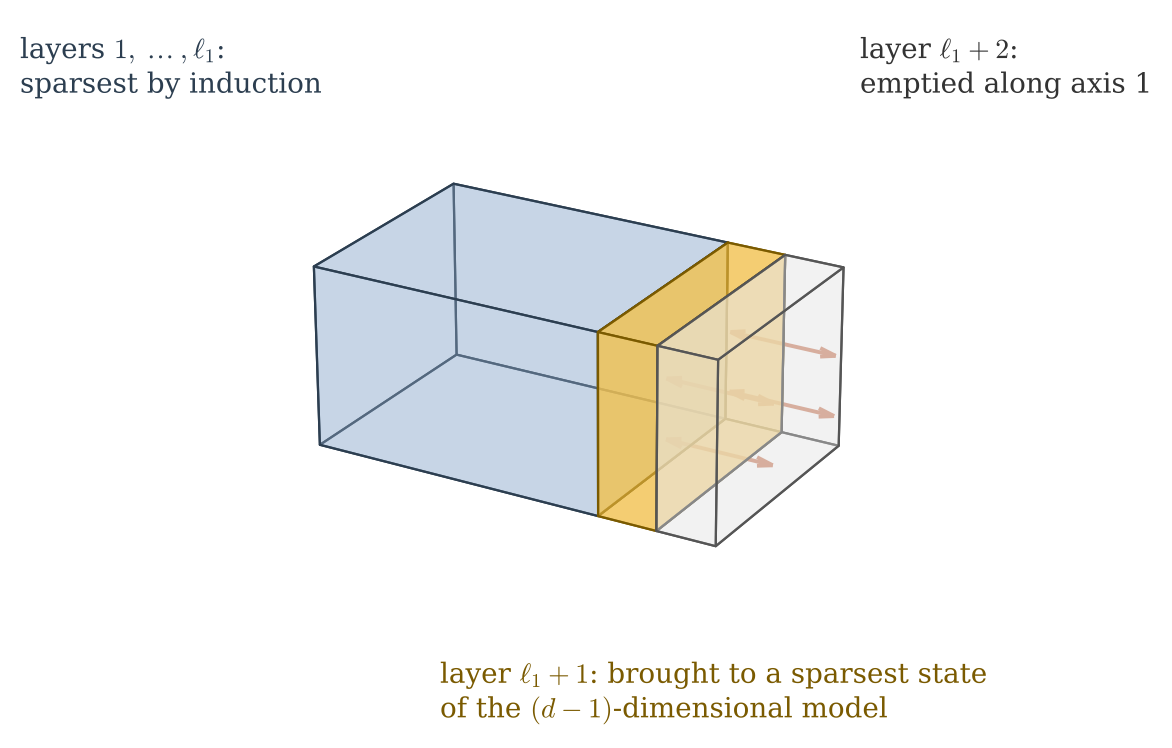
\includegraphics[width=0.66\textwidth]{fig_layers.png}
\caption{The induction step of Proposition~\ref{prop:layers}. The first $\ell_1$ layers are brought to a sparsest configuration; the last layer is emptied by toppling along axis $1$; the layer between them is reset to the full configuration and then treated as a box of dimension $d-1$.}\label{fig:layers}
\end{figure}

\begin{proposition}\label{prop:layers}
For $d\ge2$, $\ell_1\ge1$ and $\ell'=(\ell_2,\dots,\ell_d)$,
\[
\Nmin^{(d)}(\ell_1+2,\ell')\ \le\ \Nmin^{(d)}(\ell_1,\ell')+\Nmin^{(d-1)}(\ell').
\]
\end{proposition}

\begin{proof}
Write $\B'=[\ell_2]\times\dots\times[\ell_d]$, $\B_0=[\ell_1]\times\B'$, $\B=[\ell_1+2]\times\B'$, and $L_k=\{k\}\times\B'$ for the layers of $\B$. Let $z_0$ be a recurrent configuration on $\B_0$ with $\Nmin^{(d)}(\ell_1,\ell')$ grains, $\mathcal H_0$ a legal history from $\one$ to $z_0$ on $\B_0$, $z_1$ a recurrent configuration of the $(d-1)$-dimensional model on $\B'$ with $\Nmin^{(d-1)}(\ell')$ grains, and $\mathcal H_1$ a legal history from $\one$ to $z_1$ on $\B'$. We build a legal history on $\B$ from $\one$ in four stages (Figure~\ref{fig:layers}).

\emph{Stage 1.} Perform $\mathcal H_0$ on the layers $L_1,\dots,L_{\ell_1}$. The heights on these layers evolve exactly as in $\B_0$: a toppling of a site of $L_{\ell_1}$ along axis $1$ sends a grain to $L_{\ell_1+1}$ instead of out of $\B_0$, and nothing comes back, because no site of $L_{\ell_1+1}$ topples during this stage. So every toppling remains legal, and at the end $L_1,\dots,L_{\ell_1}$ carry $z_0$, while the sites of $L_{\ell_1+1}$ carry their initial grain plus what they received.

\emph{Stage 2.} For each site $s\in L_{\ell_1+2}$, add a grain at $s$ and topple $s$ along axis $1$. The toppling is legal, it empties $s$, sends one grain out of $\B$ and one to $L_{\ell_1+1}$, and it does not touch other sites of $L_{\ell_1+2}$.

\emph{Stage 3.} Topple unstable sites of $L_{\ell_1+1}$, only along axes $2,\dots,d$, until $L_{\ell_1+1}$ is stable; this terminates by Lemma~\ref{lem:finite} with $A=\{2,\dots,d\}$, and these topplings move grains only inside $L_{\ell_1+1}$ or out of $\B$. Then add a grain at each empty site of $L_{\ell_1+1}$. Now $L_{\ell_1+1}$ is full.

\emph{Stage 4.} Perform $\mathcal H_1$ on $L_{\ell_1+1}$, the axes $1,\dots,d-1$ of $\B'$ being the axes $2,\dots,d$ of $\B$. A toppling along these axes sends grains to sites of $L_{\ell_1+1}$ or out of $\B$, exactly as in $\B'$, so the history stays legal and ends with $z_1$ on $L_{\ell_1+1}$.

No stage after the first changes $L_1,\dots,L_{\ell_1}$, and none after the second changes $L_{\ell_1+2}$. The final configuration is $z_0$ on the first $\ell_1$ layers, $z_1$ on $L_{\ell_1+1}$ and $0$ on $L_{\ell_1+2}$. It is stable, it is reached from $\one$ by a legal history, so it is recurrent, and it has $\Nmin^{(d)}(\ell_1,\ell')+\Nmin^{(d-1)}(\ell')$ grains.
\end{proof}

In dimension two the layer is a column and Stage~4 is Lemma~\ref{lem:chain}; this is the construction of \cite[\S6]{Dha99b}, where the column is relaxed in one step.\footnote{Stage~3 replaces the remark in \cite[\S6]{Dha99b} that the column ``essentially'' behaves as a one-dimensional deterministic sandpile, so that at most one site of it ends empty. Resetting the layer to the full configuration first makes the bookkeeping exact in every dimension.}

\begin{proof}[Proof of Theorem~\ref{thm:B}]
The lower bound is Theorem~\ref{thm:lower}. For the upper bound we induct on $d$. For $d=1$ it is Lemma~\ref{lem:chain}. Let $d\ge2$ and suppose that at least $d-1$ of the $\ell_i$ are odd. By symmetry we may assume that $\ell_1$ is odd; then at least $d-2$ of $\ell_2,\dots,\ell_d$ are odd, and by induction $\Nmin^{(d-1)}(\ell')=2^{2-d}\prod_{i\ge2}(\ell_i-1)$. Lemma~\ref{lem:thin} and $(\ell_1-1)/2$ applications of Proposition~\ref{prop:layers} give
\[
\Nmin^{(d)}(\ell_1,\ell')\ \le\ \frac{\ell_1-1}2\,\Nmin^{(d-1)}(\ell')\ =\ 2^{1-d}\prod_{i=1}^d(\ell_i-1).\qedhere
\]
\end{proof}

\begin{proof}[Proof of Theorem~\ref{thm:A}]
The lower bound is Theorem~\ref{thm:lower} with \eqref{eq:fceil}. If $\ell$ or $m$ is odd, the upper bound is Theorem~\ref{thm:B} with $d=2$. Let $\ell$ and $m$ be even. Proposition~\ref{prop:layers}, applied along the second axis, and Lemma~\ref{lem:chain} give $\Nmin(2,m+2)\le\Nmin(2,m)+1$, so Lemma~\ref{lem:twotwo} gives $\Nmin(2,m)\le m/2$. Applied along the first axis, Proposition~\ref{prop:layers} gives $\Nmin(\ell+2,m)\le\Nmin(\ell,m)+(m-1)$, hence
\[
\Nmin(\ell,m)\ \le\ \frac m2+\frac{\ell-2}2\,(m-1)\ =\ \frac{\ell m-\ell-m+2}2\ =\ f(\ell,m).\qedhere
\]
\end{proof}

\begin{figure}[t]
\centering
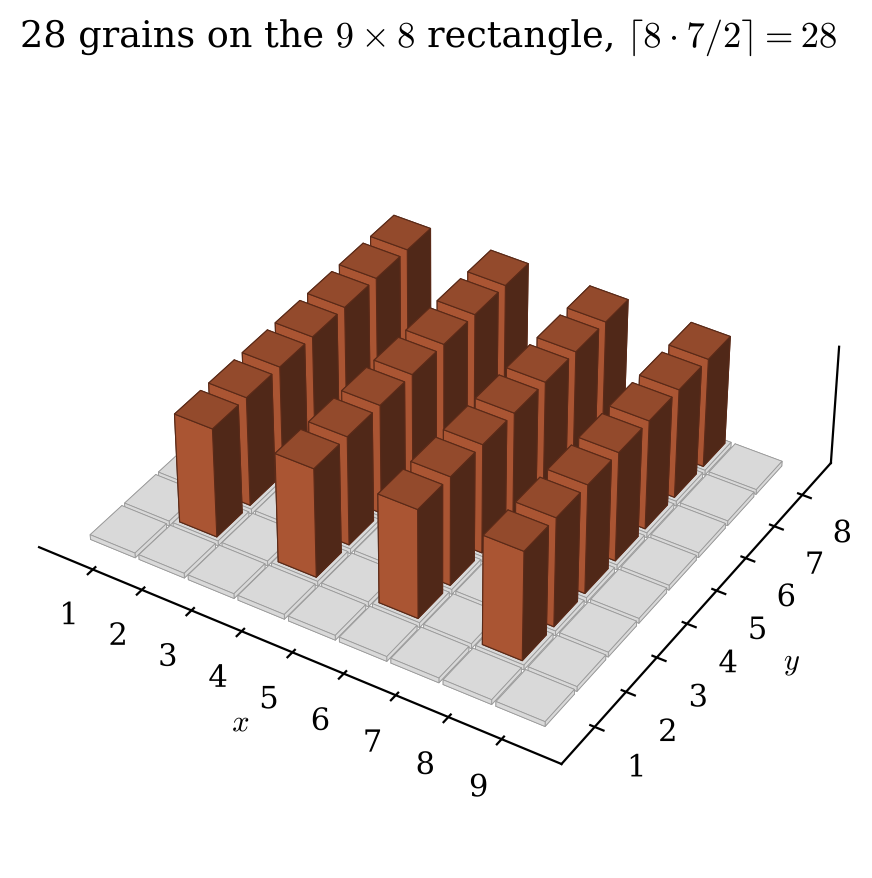
\includegraphics[width=0.66\textwidth]{fig_minimal.png}
\caption{A recurrent configuration with the fewest grains on the $9\times8$ rectangle, produced by the history of Theorem~\ref{thm:A}: the columns $x=2,4,6,8$ each carry seven grains and the odd columns are empty, $4\cdot7=28=\lceil 8\cdot7/2\rceil$.}\label{fig:minimal}
\end{figure}

For odd $\ell$ the sparsest configurations produced by the proof are easy to describe (Figure~\ref{fig:minimal}): the odd columns are empty, and each even column carries $m-1$ grains, with its empty site at the bottom, the site where Lemma~\ref{lem:chain} leaves its vacancy.\footnote{In Lemma~\ref{lem:chain} the vacancy is at the site $1$, the end opposite to the addition. Running the history of Lemma~\ref{lem:chain} from the other end, with the addition at site $1$ and topplings of $1,2,\dots,\ell$, leaves the vacancy at $\ell$ instead, so the empty site of each even column may be put at either end.} In three dimensions the same recipe empties every odd slab and fills each even slab with a sparsest two-dimensional configuration (Figure~\ref{fig:box3d}).

\begin{figure}[t]
\centering
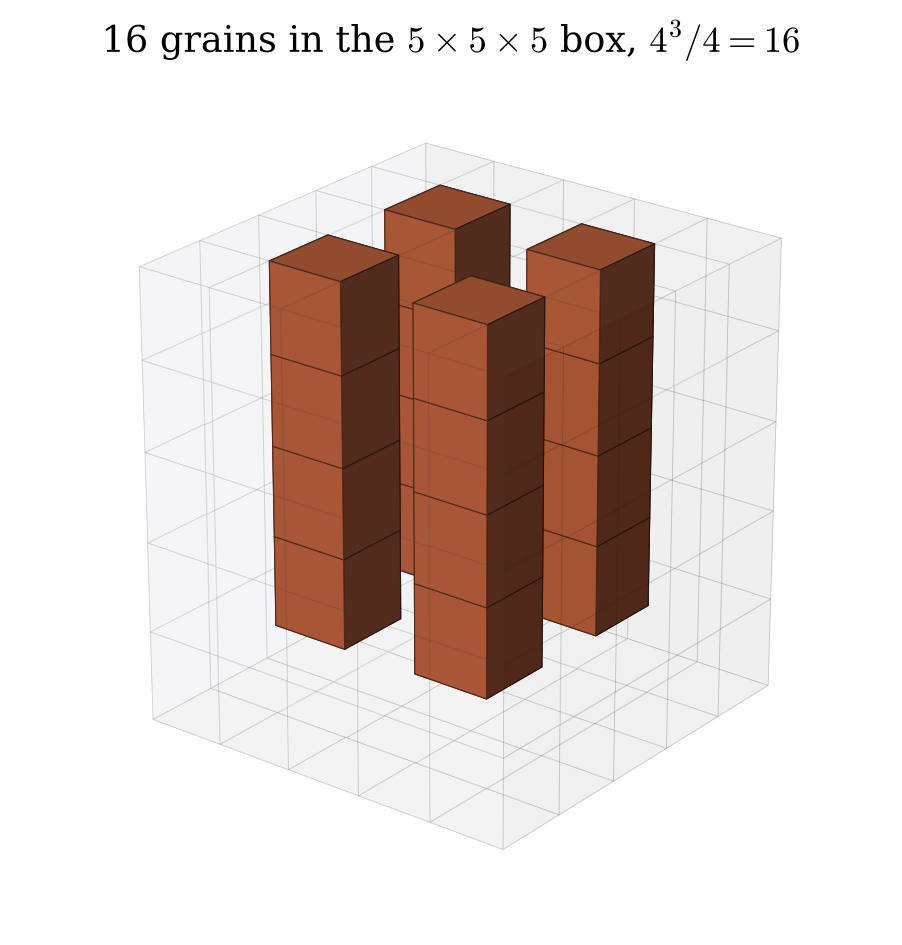
\includegraphics[width=0.58\textwidth]{fig_box3d.png}
\caption{A recurrent configuration with the fewest grains in the $5\times5\times5$ box, from the history of Theorem~\ref{thm:B}: $16=4^3/4$ grains, in two slabs, each a sparsest configuration of the $5\times5$ square.}\label{fig:box3d}
\end{figure}

\section{Further consequences and open cases}\label{sec:remarks}

\subsection{Boxes with a side equal to three}
If $\ell_1=3$, one application of Proposition~\ref{prop:layers} and Lemma~\ref{lem:thin} give $\Nmin^{(d)}(3,\ell')\le\Nmin^{(d-1)}(\ell')$, while Theorem~\ref{thm:lower} gives $\Nmin^{(d)}(3,\ell')\ge\lceil 2^{2-d}\prod_{i\ge2}(\ell_i-1)\rceil$. Whenever $\Nmin^{(d-1)}(\ell')$ equals its own lower bound, the two agree. With Theorem~\ref{thm:A} this gives, for instance,
\[
\Nmin^{(3)}(3,\ell,m)=\Bigl\lceil\tfrac12(\ell-1)(m-1)\Bigr\rceil\qquad\text{for all }\ell,m\ge1,
\]
which is not covered by Theorem~\ref{thm:B} when $\ell$ and $m$ are both even.

\subsection{Boxes with a side equal to two}
In the proof of Theorem~\ref{thm:lower} an edge along axis $i$ was allowed to lie in $2^{d-1}$ cells. If $\ell_j=2$, every cell has the same $j$-th offset, and an edge lies in at most half as many cells as the general count allows. Write a box with sides of length two as $[2]^k\times[\ell_1]\times\dots\times[\ell_{d'}]$ with $k\ge1$, $d'\ge0$ and $\ell_1,\dots,\ell_{d'}\ge3$, so that $d=k+d'$.

\begin{theorem}\label{thm:two}
Every recurrent configuration on $[2]^k\times[\ell_1]\times\dots\times[\ell_{d'}]$ has at least
\[
\Bigl\lceil 2^{-d'}\prod_{i=1}^{d'}(\ell_i-1)\Bigr\rceil
\]
grains. The bound is attained if all of $\ell_1,\dots,\ell_{d'}$ are odd, if $d'=1$, and if one of them is even and all others are equal to $3$.
\end{theorem}

\begin{lemma}\label{lem:cube}
$\Nmin^{(k)}(2,\dots,2)=1$ for every $k\ge1$.
\end{lemma}

\begin{proof}
In $[2]^k$ each site has exactly one neighbour inside the box along each axis; the other one lies outside. List the $2^k$ sites as $v_0,v_1,\dots,v_{2^k-1}$ so that $v_j$ and $v_{j+1}$ are neighbours for every $j$, indices taken modulo $2^k$; for $k\ge2$ the reflected Gray code gives such a cycle, and for $k=1$ take $v_0=1$, $v_1=2$. From $\one$, add a grain at $v_0$ and topple $v_0,v_1,\dots,v_{2^k-1}$ in this order, each $v_j$ along the axis of the edge $\{v_j,v_{j+1}\}$. When $v_j$ topples it holds two grains, its own and the one it has just received; it sends one to $v_{j+1}$ and one out of the box. The last toppling returns a grain to $v_0$, which had become empty. Every site has toppled once, and one grain remains, at $v_0$. The lower bound $1$ is Theorem~\ref{thm:lower} applied to the single cell.
\end{proof}

\begin{proof}[Proof of Theorem~\ref{thm:two}]
\emph{Lower bound.} Repeat the proof of Theorem~\ref{thm:lower} with $\B'=\B$. A cell is determined by its offsets in the $d'$ long directions, so there are $\prod_i(\ell_i-1)$ cells. An edge along any axis lies in at most $2^{d'}$ cells: its coordinates in the $d'$ long directions, other than its own axis, admit at most two offsets each, and those in the short directions admit one. Each site lies in at most $2^{d'}$ cells and each cell has $2^d$ corners, so the cells of Case~2 number at most $2^{d'-d}|U|\le|U|$. Hence
\[
\prod_i(\ell_i-1)\ \le\ 2^{d'}\sum_{u\in T}z(u)+\sum_{u\in U}z(u)\ \le\ 2^{d'}\sum_{s\in\B}z(s).
\]

\emph{Upper bound.} By Lemma~\ref{lem:thin} and Proposition~\ref{prop:layers} applied along an odd axis $\ell_i$, the minimum on the box is at most $\tfrac12(\ell_i-1)$ times the minimum on the box with that side removed. If all $\ell_i$ are odd, removing them one by one and ending with Lemma~\ref{lem:cube} gives $2^{-d'}\prod_i(\ell_i-1)$, the lower bound. For $d'=1$ and $\ell_1=m$, Proposition~\ref{prop:layers} along the last axis gives $\Nmin([2]^k,m+2)\le\Nmin([2]^k,m)+\Nmin([2]^k)=\Nmin([2]^k,m)+1$ by Lemma~\ref{lem:cube}. Starting from $\Nmin([2]^k,1)=0$ for odd $m$, and from $\Nmin([2]^k,2)=\Nmin([2]^{k+1})=1$ for even $m$, this gives $\Nmin([2]^k,m)\le\lceil(m-1)/2\rceil$, the lower bound. If one side $m$ is even and the others equal $3$, removing the sides equal to $3$ costs a factor $1$ each, so the minimum is at most $\lceil(m-1)/2\rceil=m/2$, while the lower bound is $\lceil 2^{-d'}2^{d'-1}(m-1)\rceil=m/2$.
\end{proof}

For instance $\Nmin(4,2,2)=\lceil3/2\rceil=2$, whereas Theorem~\ref{thm:B} gives only $1$, and $\Nmin(5,2,2)=2$. The exhaustive search of Appendix~\ref{app:check} confirms the values $1$, $1$ and $2$ on the boxes $2\times2\times2$, $3\times2\times2$ and $4\times2\times2$.

\subsection{The minimal density in every box}
For boxes not covered by Theorems~\ref{thm:B} and~\ref{thm:two} the constructions still give the right density.

\begin{proposition}\label{prop:density}
For every box,
\[
\Bigl|\,\Nmin(\ell_1,\dots,\ell_d)-2^{1-d}\prod_i\ell_i\,\Bigr|\ \le\ 2\sum_{j=1}^d\ \prod_{i\ne j}\ell_i .
\]
In particular $\Nmin(\ell_1,\dots,\ell_d)/\prod_i\ell_i\to2^{1-d}$ as $\min_i\ell_i\to\infty$.
\end{proposition}

\begin{proof}
Write $\Sigma(\ell)=\sum_j\prod_{i\ne j}\ell_i$. For the upper bound we show $\Nmin\le2^{1-d}\prod_i\ell_i+2\Sigma(\ell)$ by induction on $d$. For $d=1$, $\Nmin(\ell)=\ell-1\le\ell+2$. Let $d\ge2$. The configuration $\one$ is recurrent, so $\Nmin(2,\ell')\le2\prod_{i\ge2}\ell_i$; with $\Nmin(1,\ell')=0$ and Proposition~\ref{prop:layers}, for $\ell_1$ of either parity
\[
\Nmin(\ell_1,\ell')\ \le\ 2\prod_{i\ge2}\ell_i+\frac{\ell_1}2\,\Nmin^{(d-1)}(\ell')\ \le\ 2\prod_{i\ge2}\ell_i+2^{1-d}\prod_i\ell_i+\sum_{j\ge2}\prod_{i\ne j}\ell_i,
\]
using the induction hypothesis $\Nmin^{(d-1)}(\ell')\le2^{2-d}\prod_{i\ge2}\ell_i+2\sum_{j\ge2}\prod_{i\ge2,\,i\ne j}\ell_i$. The right side is at most $2^{1-d}\prod_i\ell_i+2\Sigma(\ell)$. For the lower bound, the inequality $\prod_i(1-a_i)\ge1-\sum_ia_i$ for $0\le a_i\le1$ (multiply $\prod_{i<n}(1-a_i)\ge1-\sum_{i<n}a_i$ by $1-a_n$ and drop the term $a_n\sum_{i<n}a_i\ge0$), applied with $a_i=1/\ell_i$, gives $\prod_i(\ell_i-1)\ge\prod_i\ell_i-\Sigma(\ell)$, so Theorem~\ref{thm:lower} gives $\Nmin\ge2^{1-d}\prod_i\ell_i-2^{1-d}\Sigma(\ell)$.
\end{proof}

\subsection{Open cases}
Theorems~\ref{thm:B} and~\ref{thm:two} and the case of a side equal to $3$ do not settle every box of dimension three or more. On $2\times4\times4$ Theorem~\ref{thm:two} gives $3\le\Nmin$ and Proposition~\ref{prop:layers} along the second axis gives $\Nmin(2,4,4)\le\Nmin(2,2,4)+\Nmin(2,4)=4$; on $4\times4\times5$ the bounds are $9$ and $10$. All values computed so far agree with the following rule. For a box with all sides at least $2$, let $M=2^{d-1}$ if every side is at least $3$, and $M=2^{d'}$ if exactly $d'$ sides are at least $3$ and the others equal $2$.

\begin{question}
Is $\Nmin(\ell_1,\dots,\ell_d)=\bigl\lceil\prod_i(\ell_i-1)/M\bigr\rceil$ for every box with all sides at least $2$?
\end{question}

\subsection{Cylinders}
Dhar also considered periodic boundary conditions in one direction \cite[\S\S3--4]{Dha99b}. On the cylinder $[\ell]\times\ZZ/m\ZZ$ with $m\ge3$, open in the first direction and periodic in the second, Lemma~\ref{lem:finite} fails for topplings along the periodic axis alone, since they never lose a grain, but its conclusion holds almost surely for the chain: each toppling is horizontal with probability $\tfrac12$, independently of the past, so a site that topples infinitely often almost surely topples horizontally infinitely often, and the argument of Lemma~\ref{lem:finite} run along the first axis gives a contradiction. The proof of Lemma~\ref{lem:recurrent} then applies unchanged, a recurrent configuration is the end point of a finite legal history from $\one$, and the proof of Theorem~\ref{thm:lower}, applied to the $(\ell-1)m$ unit squares, shows that every recurrent configuration has at least $\lceil(\ell-1)m/2\rceil$ grains. The construction of Section~\ref{sec:upper} does not carry over: Stage~3 needs the sites of a column to lose grains when they topple vertically, and a periodic column loses none. Indeed, the configuration with full even columns and empty odd columns is not recurrent on the $3\times4$ cylinder. The exhaustive search shows that the lower bound is attained on every cylinder with $\ell\ge2$, $m\ge3$ and $\ell m\le12$, and on $3\times5$. Whether $\lceil(\ell-1)m/2\rceil$ is the minimum on every cylinder we leave open.

\subsection{On Dhar's paper}
Our checks of \cite{Dha99b} confirm its statements. A pattern that occurs in no recurrent configuration of its bounding box occurs in no recurrent configuration of any larger box: if a legal history from $\one$ on the larger box is restricted to the sites of a sub-box, and the grains entering the sub-box from outside are counted as additions, the result is a legal history on the sub-box, so the restriction of a recurrent configuration is recurrent. With this, a search over the bounding boxes shows that the patterns of Figure~1 of \cite{Dha99b} are forbidden and that the pattern of its Figure~2 occurs in recurrent configurations, as claimed; the modified burning test burns Figure~1d completely and does not burn Figure~2, as stated there. Every configuration of the $2\times2$ square other than the empty one is recurrent, and on $2\times3$ the transient configurations are exactly those containing an empty unit square. The text has a few misprints that do not affect its content.\footnote{In \cite[\S6]{Dha99b} the formula for $f$ is \cite[(23)]{Dha99b} but is referred to as eq.~(20), and the conjecture is \cite[(22)]{Dha99b} but is referred to as eq.~(18); the rectangle ``$0\le x\le\ell_0$, $0\le y\le m_0$'' should read $1\le x\le\ell_0$, $1\le y\le m_0$; and the increment of the grain count in the induction step is $m_0-1$, written $m-1$.} Theorem~\ref{thm:A} confirms the value $\rho_{\min}=\tfrac12$ that Dhar predicted, and Theorem~\ref{thm:lower} shows more: the half-density bound holds in every window, not only on average. The author's earlier work on lattices, group actions and the geometry of K3 and Calabi--Yau manifolds is in \cite{BBS23,Bha22,BN26,Bha22b}.

\appendix

\section{An exhaustive check}\label{app:check}

The proofs above use no computation. As an independent check, the set of recurrent configurations was computed on small rectangles by a breadth-first search from $\one$, using the criterion after Lemma~\ref{lem:realize}. For each stable configuration reached and each site, a grain is added and all outcomes of the relaxation are generated by toppling the smallest unstable site along each of the two axes in turn. With the sites ordered as in the program, these are exactly the stable configurations that one step of the chain reaches with positive probability, and by Lemma~\ref{lem:realize} the recurrent set does not depend on the order. The search gives $15$ recurrent configurations out of $16$ on the $2\times2$ square, $57$ of $64$ on $2\times3$, $819$ of $1024$ on $2\times5$, $410$ of $512$ on $3\times3$, $2945$ of $4096$ on $3\times4$, $21158$ of $32768$ on $3\times5$ and $40047$ of $65536$ on $4\times4$. In every case the least number of grains is $f(\ell,m)$, in agreement with Theorem~\ref{thm:A} and with Dhar's checks for $\ell,m\le4$ \cite[\S6]{Dha99b}. The same search in three dimensions, where each unstable site is toppled along each of the three axes in turn, gives $255$ recurrent configurations of $256$ on $2\times2\times2$, $4065$ of $4096$ on $3\times2\times2$ and $64800$ of $65536$ on $4\times2\times2$, with least numbers of grains $1$, $1$ and $2$, as Theorem~\ref{thm:two} predicts. On cylinders $[\ell]\times\ZZ/m\ZZ$ it gives $54$ of $64$ on $2\times3$, $207$ of $256$ on $2\times4$, $783$ of $1024$ on $2\times5$, $2970$ of $4096$ on $2\times6$, $364$ of $512$ on $3\times3$, $2669$ of $4096$ on $3\times4$, $19124$ of $32768$ on $3\times5$ and $2427$ of $4096$ on $4\times3$, with least numbers of grains $\lceil(\ell-1)m/2\rceil$ in each case. The legal histories of Section~\ref{sec:upper} were also executed literally, with every toppling tested for legality, on boxes of dimensions one to four; each ends at a stable configuration with the number of grains given by Theorems~\ref{thm:A}, \ref{thm:B} and~\ref{thm:two}, and on the small rectangles above the configuration it produces lies in the computed recurrent set.

\section*{Declarations}

\subsection*{Data availability}
All results are proved in the article. The programs of Appendix~\ref{app:check}, which repeat the exhaustive check and the constructions and draw the figures, are archived at doi:\zenodoCodeDOI.

\subsection*{Funding}
None.

\subsection*{Conflict of interest}
None.

\subsection*{Ethics statement}
This study involves no human participants, animals or personal data; no ethical approval was required.

\begin{thebibliography}{99}\raggedright

\bibitem{BTW87} P.~Bak, C.~Tang, K.~Wiesenfeld, \emph{Self-organized criticality: an explanation of the $1/f$ noise}, Phys. Rev. Lett. \textbf{59} (1987), 381--384. doi:10.1103/PhysRevLett.59.381

\bibitem{BTW88} P.~Bak, C.~Tang, K.~Wiesenfeld, \emph{Self-organized criticality}, Phys. Rev. A \textbf{38} (1988), 364--374. doi:10.1103/PhysRevA.38.364

\bibitem{BBS23} D.~Bhattacharjee, P.~Bose, P.~Samal, \emph{Ramanujan $\tau$-function and its relationship with $PSL(2,\mathbb Z)$ for $\mathcal L_{24}(\tau)^{+,E}$}, Research Square (2023). doi:10.21203/rs.3.rs-2796280/v1

\bibitem{Bha22} D.~Bhattacharjee, \emph{Generalization of quartic and quintic Calabi--Yau manifolds fibered by polarized K3 surfaces}, Research Square (2022). doi:10.21203/rs.3.rs-1965255/v1

\bibitem{Bha22b} D.~Bhattacharjee, \emph{Establishing equivariant class $[O]$ for hyperbolic groups}, Asian Res. J. Math. \textbf{18} (2022), no.~11, 362--369. doi:10.9734/arjom/2022/v18i11615

\bibitem{BN26} D.~Bhattacharjee, P.~Nandi, \emph{Enriques and Kummer surfaces arising from K3 involutions}, Preprints (2026). doi:10.20944/preprints202602.0098.v1

\bibitem{BL16} B.~Bond, L.~Levine, \emph{Abelian networks I. Foundations and examples}, SIAM J. Discrete Math. \textbf{30} (2016), 856--874. doi:10.1137/15M1030984

\bibitem{Dha90} D.~Dhar, \emph{Self-organized critical state of sandpile automaton models}, Phys. Rev. Lett. \textbf{64} (1990), 1613--1616. doi:10.1103/PhysRevLett.64.1613

\bibitem{Dha99a} D.~Dhar, \emph{The Abelian sandpile and related models}, Physica A \textbf{263} (1999), 4--25. doi:10.1016/S0378-4371(98)00493-2

\bibitem{Dha99b} D.~Dhar, \emph{Some results and a conjecture for Manna's stochastic sandpile model}, Physica A \textbf{270} (1999), 69--81. doi:10.1016/S0378-4371(99)00149-1

\bibitem{FLP10} A.~Fey, L.~Levine, Y.~Peres, \emph{Growth rates and explosions in sandpiles}, J. Stat. Phys. \textbf{138} (2010), 143--159. doi:10.1007/s10955-009-9899-6

\bibitem{MD92} S.~N.~Majumdar, D.~Dhar, \emph{Equivalence between the Abelian sandpile model and the $q\to0$ limit of the Potts model}, Physica A \textbf{185} (1992), 129--145. doi:10.1016/0378-4371(92)90447-X

\bibitem{Man91} S.~S.~Manna, \emph{Two-state model of self-organized criticality}, J. Phys. A: Math. Gen. \textbf{24} (1991), L363--L369. doi:10.1088/0305-4470/24/7/009

\bibitem{Nor97} J.~R.~Norris, \emph{Markov Chains}, Cambridge University Press, Cambridge, 1997. doi:10.1017/CBO9780511810633

\end{thebibliography}

\end{document}
